\clearpage
\subsectionold{MSVC + \olly}
\myindex{\olly}

Proviamo ad analizzare l'esempio con \olly.
Carichiamo l'eseguibile e premiamo F8 (\stepover) fino a raggiungere il nostro eseguibile invece che \TT{ntdll.dll}.
Scorriamo verso l'alto finche' appare \main .

Clicchiamo sulla prima istruzione (\TT{PUSH EBP}), premiamo F2 (\IT{set a breakpoint}), e quindi F9 (\IT{Run}).
Il breakpoint sara' scatenato all'inizio della funzione \main .

Tracciamo adesso fino al punto in cui viene calcolato l'indirizzo della variabile $x$:

\begin{figure}[H]
\centering
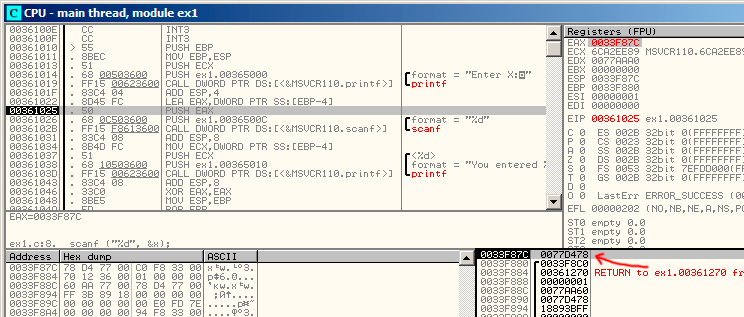
\includegraphics[scale=\FigScale]{patterns/04_scanf/1_simple/ex1_olly_1.png}
\caption{\olly: The address of the local variable is calculated}
\label{fig:scanf_ex1_olly_1}
\end{figure}


Click di destra su \EAX nella finestra dei registri e selezioniamo \q{Follow in stack}.

Questo indirizzo apparira' nella finestra dello stack.
La freccia rossa aggiunta punta alla variabile nello stack locale.
Al momento questa locazione contiene un po' di immondizia (garbage) (\TT{0x6E494714}).
Con l'aiuto dell'istruzione \PUSH l'indirizzo di questo elemento dello stack sara' memorizzato nello stesso stack alla posizione successiva.
Tracciamo con F8 finche' non viene completata l'esecuzione della funzione \scanf.
Durante l'esecuzione di \scanf, diamo in input un valore nella console. Ad esempio 123:

\begin{figure}[H]
\centering
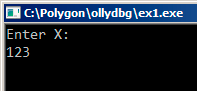
\includegraphics[scale=\NormalScale]{patterns/04_scanf/1_simple/ex1_olly_2.png}
\caption{User input in the console window}
\label{fig:scanf_ex1_olly_2}
\end{figure}

\clearpage
\scanf ha gia' completato la sua esecuzione:

\begin{figure}[H]
\centering
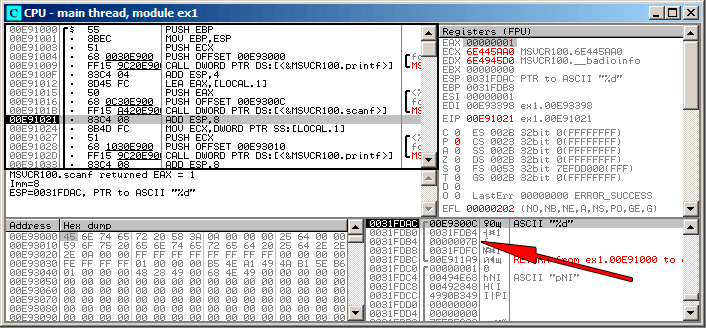
\includegraphics[scale=\FigScale]{patterns/04_scanf/1_simple/ex1_olly_3.png}
\caption{\olly: \scanf executed}
\label{fig:scanf_ex1_olly_3}
\end{figure}

\scanf restituisce 1 in \EAX, e cio' implica che ha letto con successo un valore.
Se guardiamo nuovamente l'elemento nello stack corrispondente alla variabile locale, adesso contiente \TT{0x7B} (123).

\clearpage

Successivamente questo valore viene copiato dallo stack al registro \ECX e passato a \printf:

\begin{figure}[H]
\centering
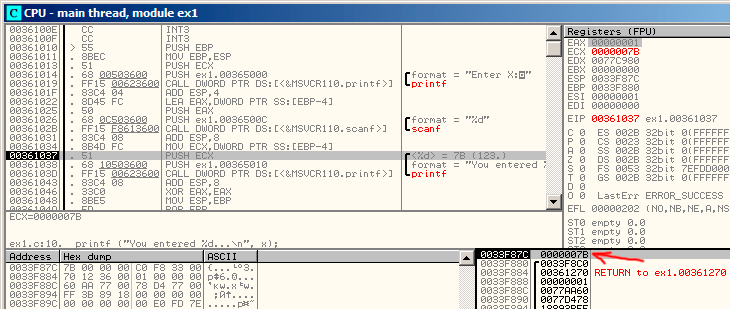
\includegraphics[scale=\FigScale]{patterns/04_scanf/1_simple/ex1_olly_4.png}
\caption{\olly: preparing the value for passing to \printf}
\label{fig:scanf_ex1_olly_4}
\end{figure}
